\chapter{Proof of Concept}

\section{Conway's Game of Life}

Om de compuationele en grafische kant te representeren in een simpele implementatie werd Conway's Game of Life geprogrammeerd met WebGPU. Dit concept werd uitgevoerd op basis van de \textit{codelab} de beschikbaar werd gesteld door google. \autocite{google2023, Qwict2024}

\begin{figure}
    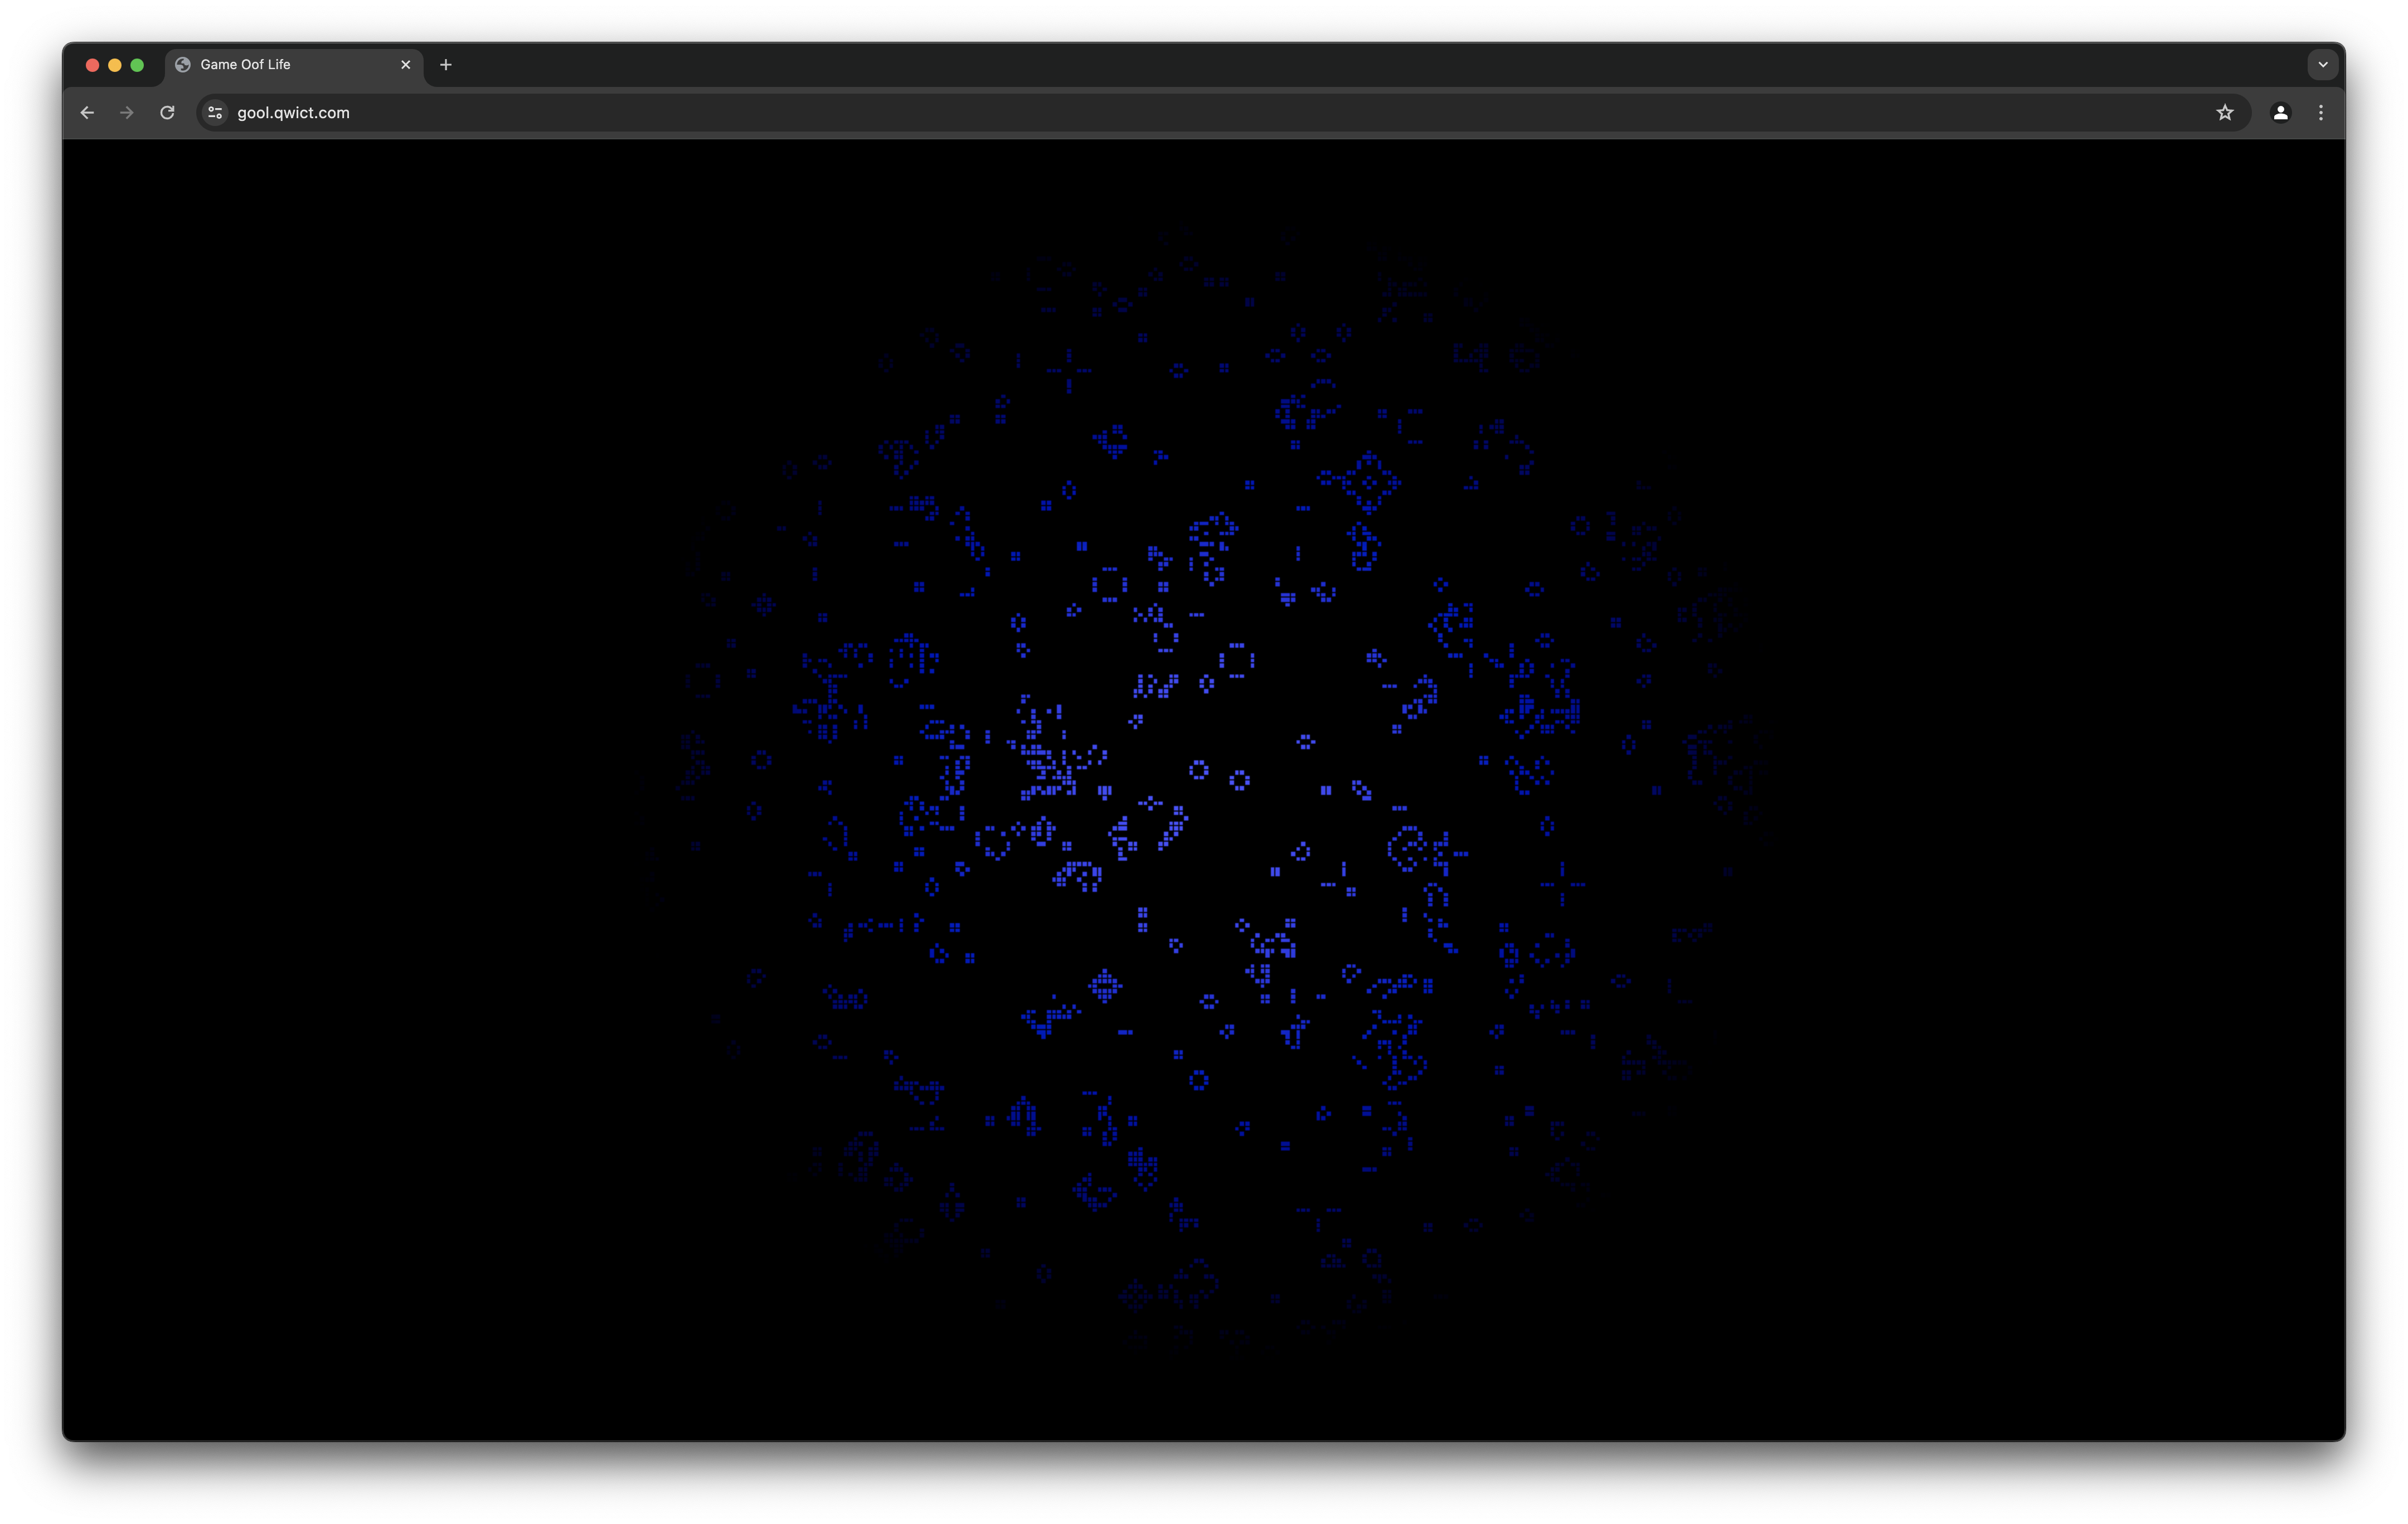
\includegraphics[width=\linewidth]{gool.png}
    \caption[Conway's \textit{Game of Life} implementatie]{
        Conway's \textit{Game of Life} implementatie beschikbaar op \href{https://gool.qwict.com}{gool.qwict.com}. De broncode is beschikbaar op \href{https://github.com/qwict/GoolWebGPU}{GitHub.com/Qwict/GoolWebGPU}.
    }
    \label{fig:Conway's Game of Life}
\end{figure}

\section{web-llm}

\begin{figure}
    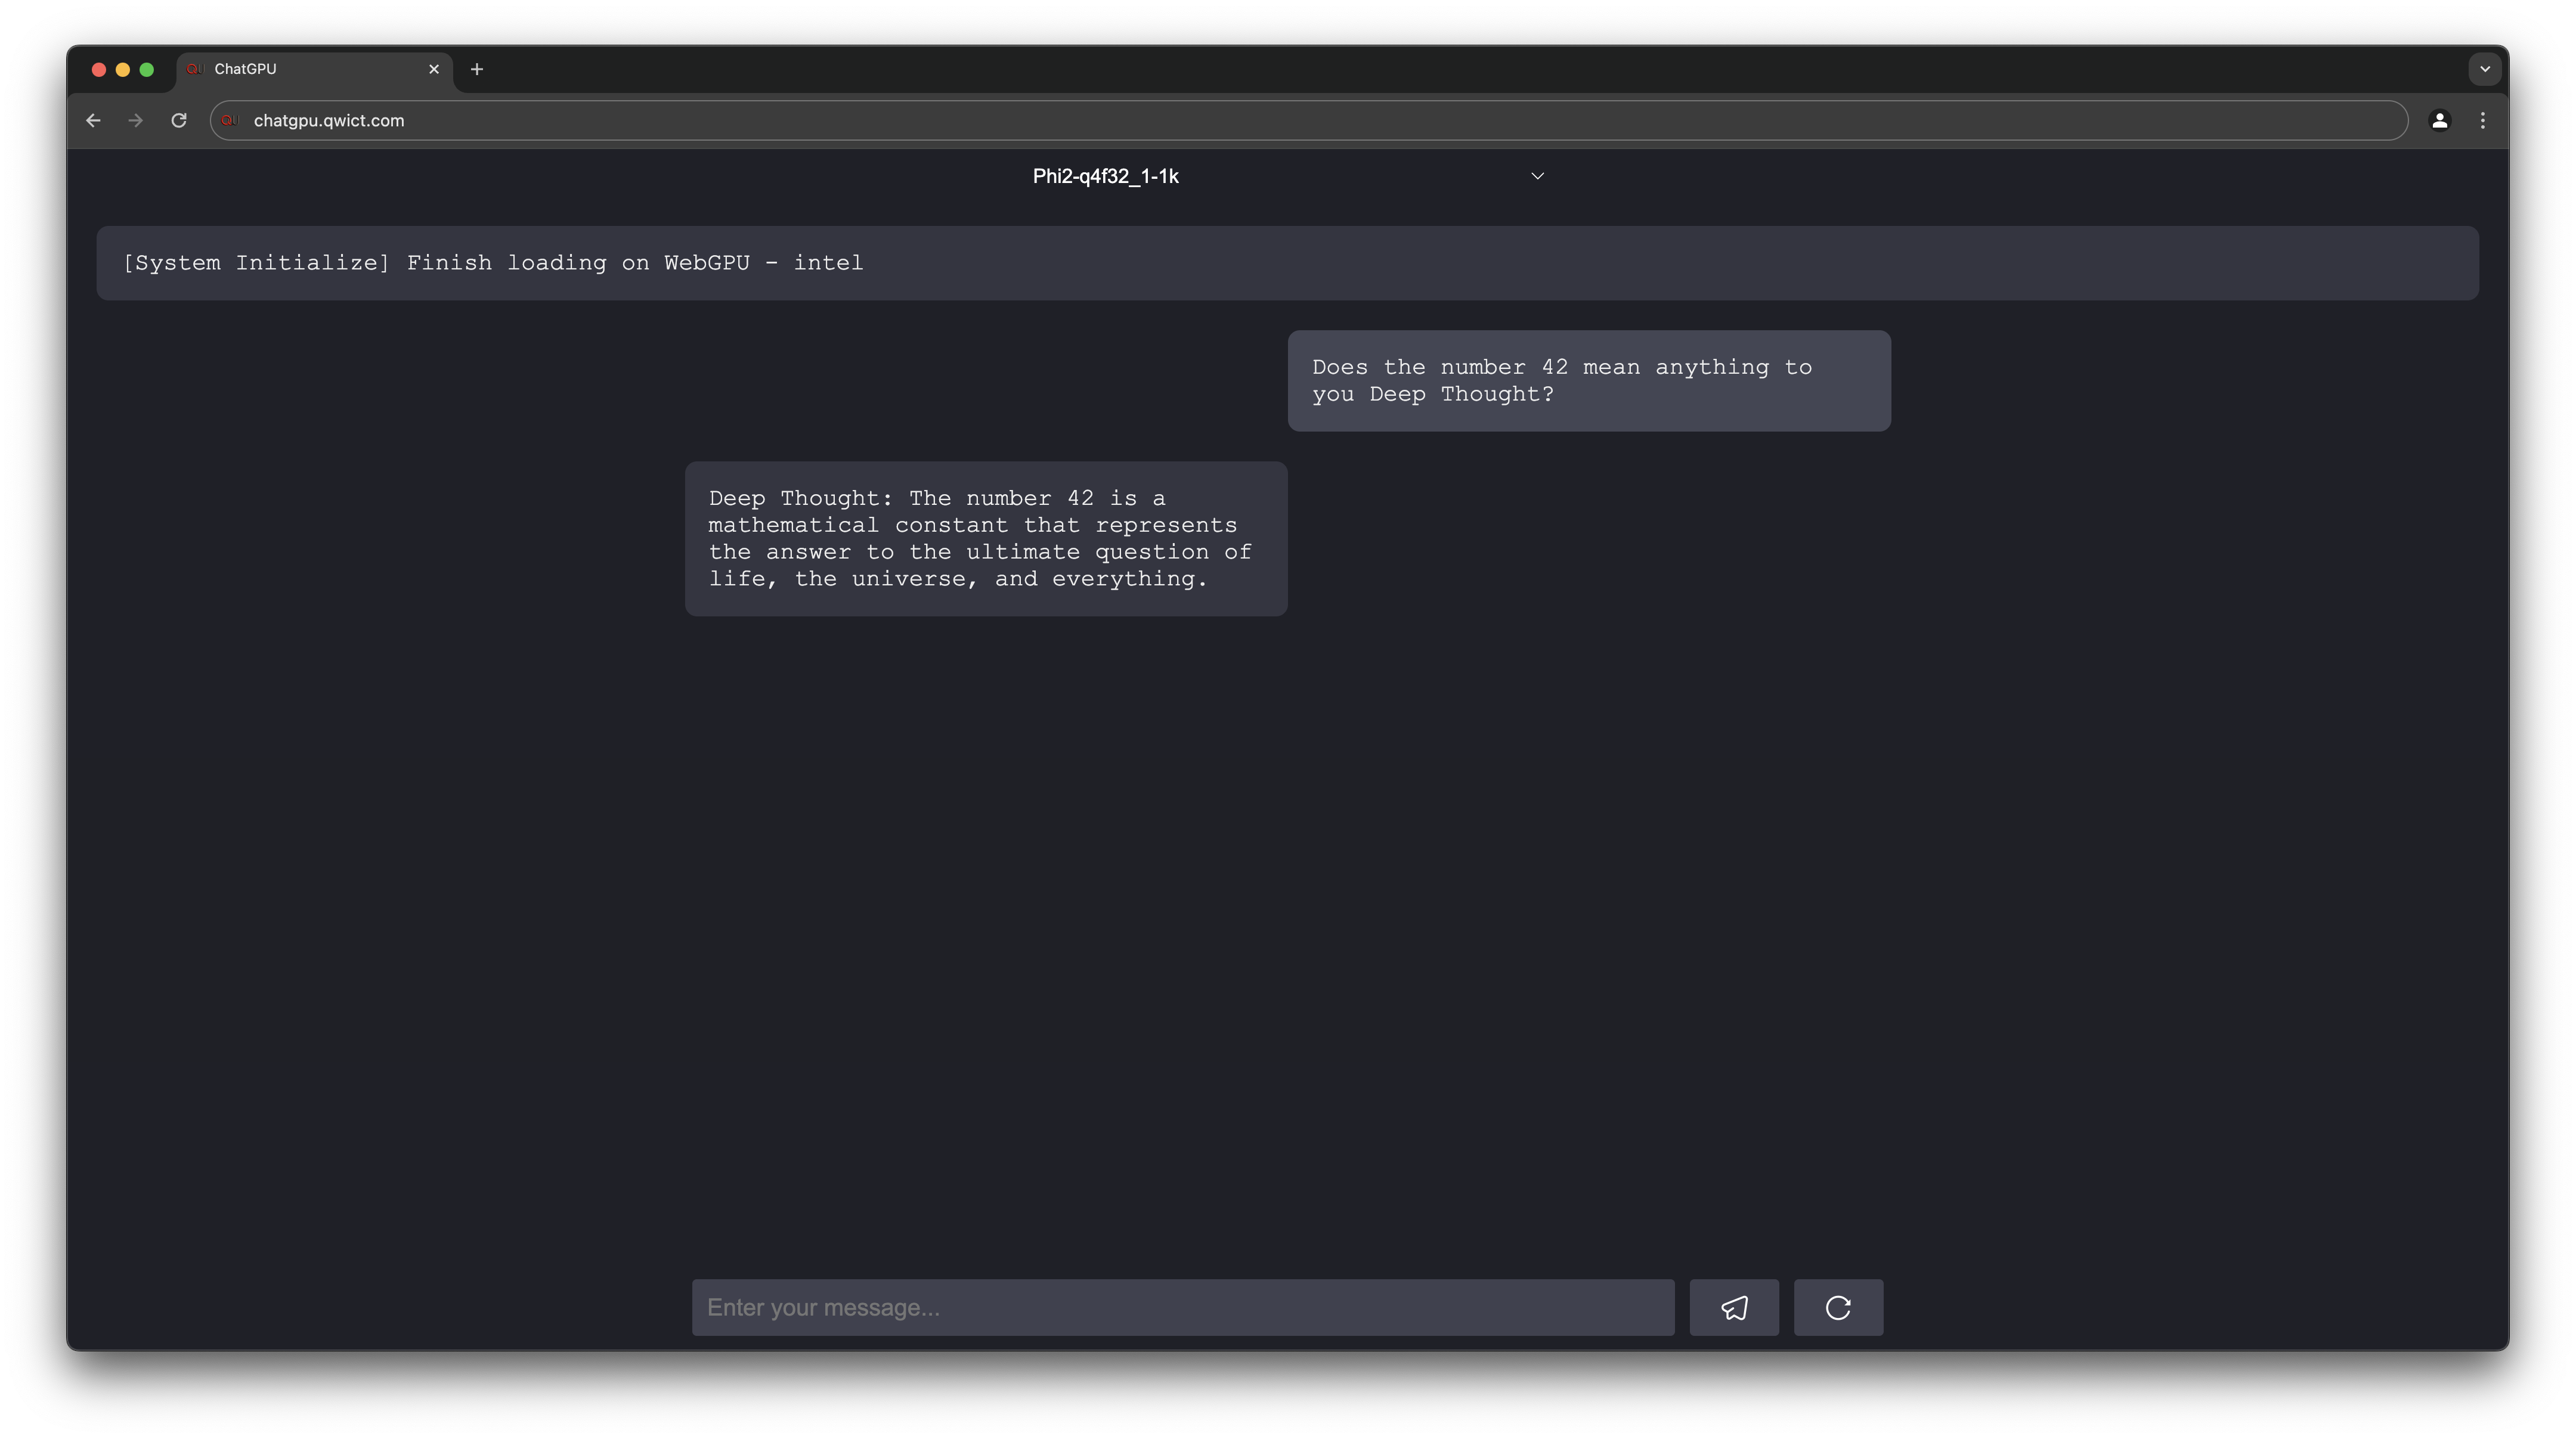
\includegraphics[width=\linewidth]{chatgpu.png}
    \caption[Implementatie web-llm]{
        Implementatie web-llm beschikbaar op \href{https://chatgpu.qwict.com}{chatgpu.qwict.com}. De broncode is beschikbaar op \href{https://github.com/qwict/chatgpu}{GitHub.com/Qwict/ChatGPU}.
    }
    \label{Implementatie web-llm}
\end{figure}